\section{Przeprowadzone testy}

Do testów zostanie wykorzystana mapa o rozmiarze 35x35 bloków.

\subsection{Wpływ ustawień na wyznaczoną ścieżkę}

W pierwszym eksperymencie został włączony skok po
przekątnej i korekcja wynikająca z tego błędów.

\begin{figure}[H]
	\centering
	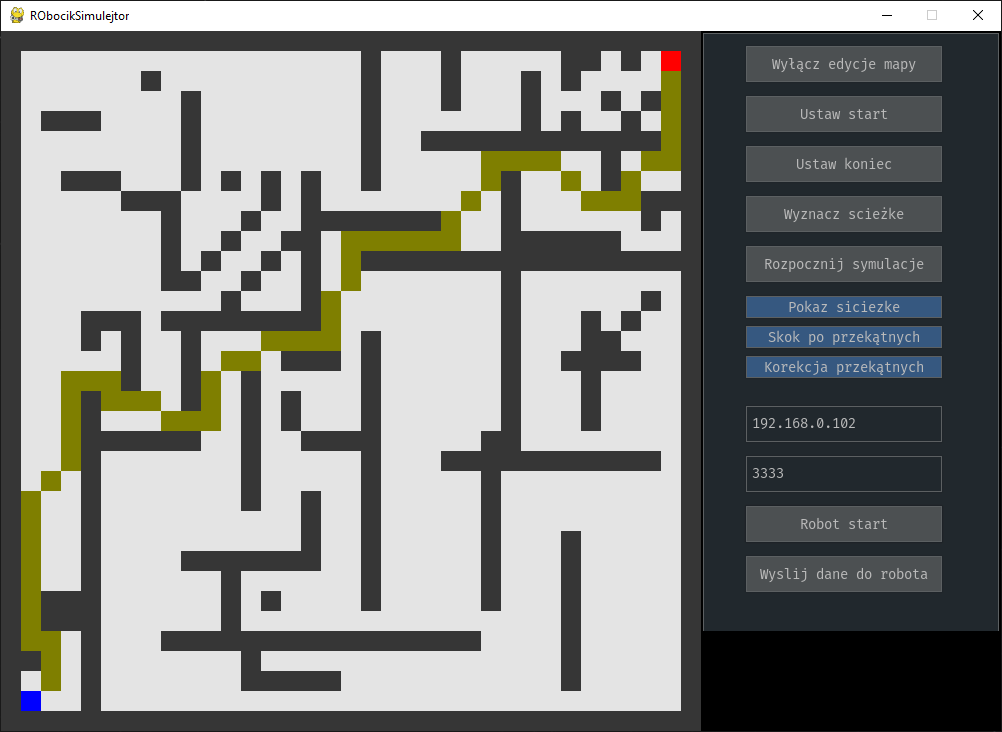
\includegraphics[width=9.5cm]{pages/testy/zdjecia/t2_1.png}
	\caption{Wyznaczona ścieżka, włączona korekcja i przejście po przekątnej}
\end{figure}

Jak widać na powyższym zdjęciu punkt docelowy został osiągnięty i robot przejechał po wyznaczonej ścieżce.
Dzięki wymienionym wcześniej opcjom robot tam gdzie to jest możliwe przejeżdża po skosie i zmniejsza czas przejazdu. 

W kolejnym teście została wyłączona korekcja przekątnych.
\begin{figure}[H]
	\centering
	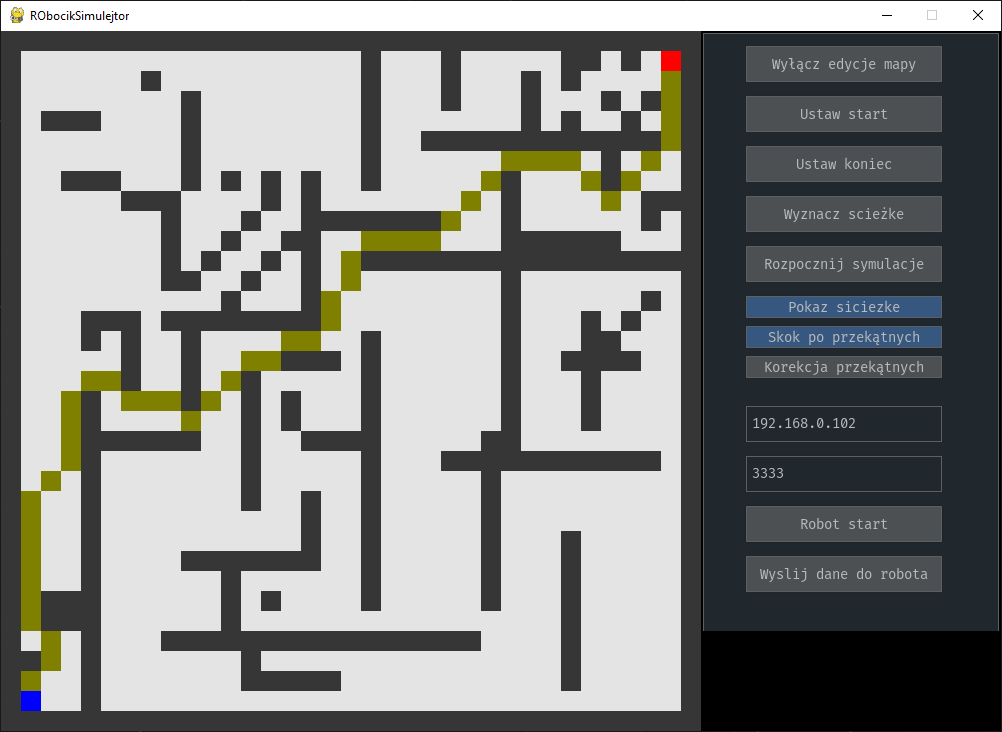
\includegraphics[width=9.5cm]{pages/testy/zdjecia/t2_2.png}
	\caption{Wyznaczona ścieżka, korekcja przekątnych jest wyłączona}
\end{figure}

Jak widać ścieżka znacząco zmieniła się w porównaniu do poprzedniego rozwiązania. Teoretycznie została wyznaczona najkrótsza 
ścieżka, jednak w praktyce robot nie byłby w stanie jej przejechać. 
W niektórych przypadkach skoku widać że robot nie miałby miejsca na przejazd.

W poniższym przypadku ścieżka trasowana bez przejścia po przekątnych. 

\begin{figure}[H]
	\centering
	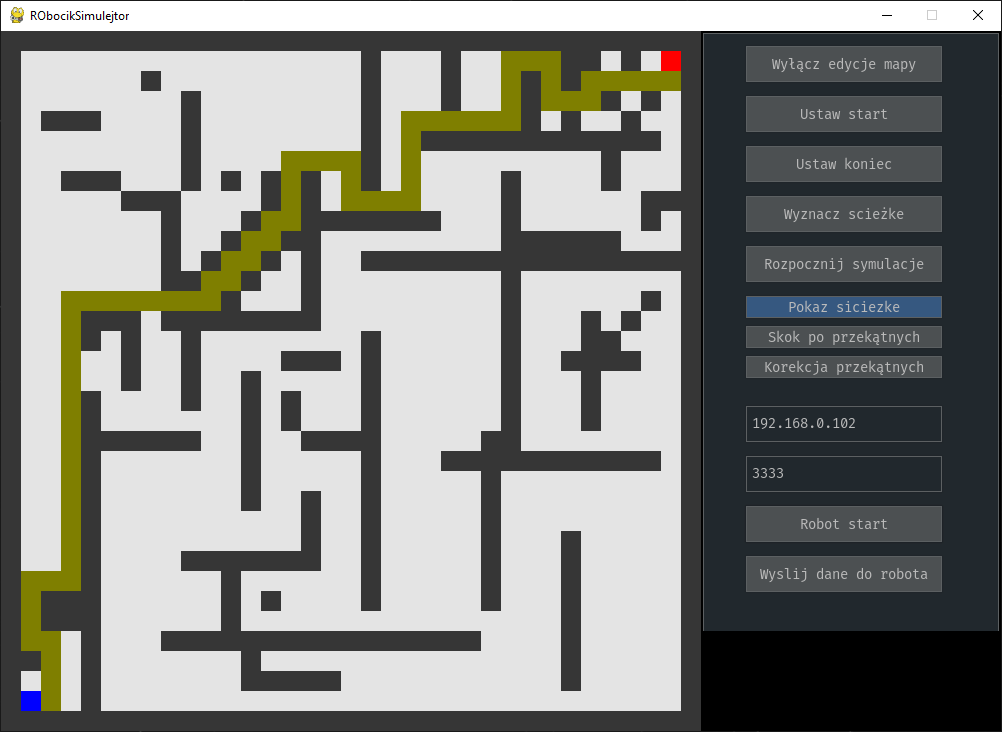
\includegraphics[width=11cm]{pages/testy/zdjecia/t2_3.png}
	\caption{Najkrótsza trasa, wyłączone przejście po przekątnych}
\end{figure}
Porównując wynik do obu poprzednich przypadków widzimy że algorytm znacznie zmienił trasę po, której przejeżdża robot
i przechodzi do następnego sąsiada tylko na wprost a więc w tym przypadku będzie najwięcej skoków.

\clearpage
\subsection{Sprawdzenie wpływu funkcji heurestycznej na ścieżkę}
Poniższy test będzie miał za zadanie sprawdzić wpływ wybranej funkcji heurestycznej na wygenerowaną ścieżkę.
\subsubsection{Funkcja Eukalidesowa}
W pierwszej kolejności zostanie sprawdzona domyślna wybrana funkcja heurestyczna opisana wzorem \eqref{Eq:heuresticEucalides}.
Rezultat działania algorytmu widoczny jest poniżej.


\textbf{Jednokrotne wzmocnienie}
\begin{figure}[H]
	\centering
	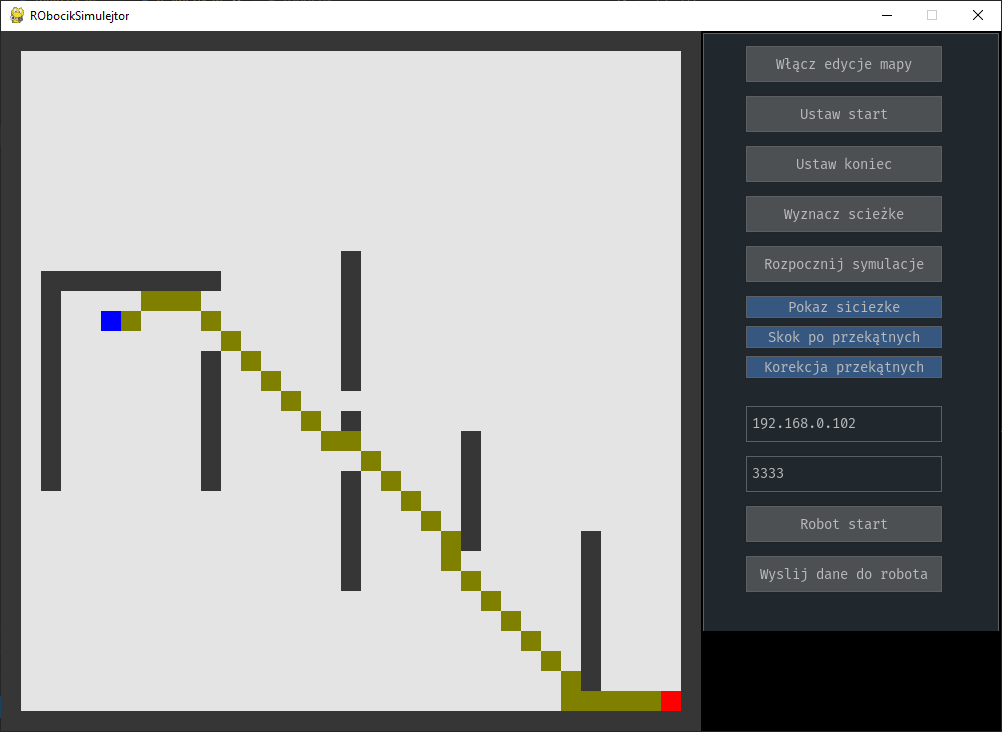
\includegraphics[width=9cm]{pages/testy/zdjecia/test3_ekualides_k1.png}
	\caption{Wyznaczona ścieżka, funkcja Eukalidesowa k=1}
\end{figure}
\textbf{Dziesięciokrotne wzmocnienie}

\begin{figure}[H]
	\centering
	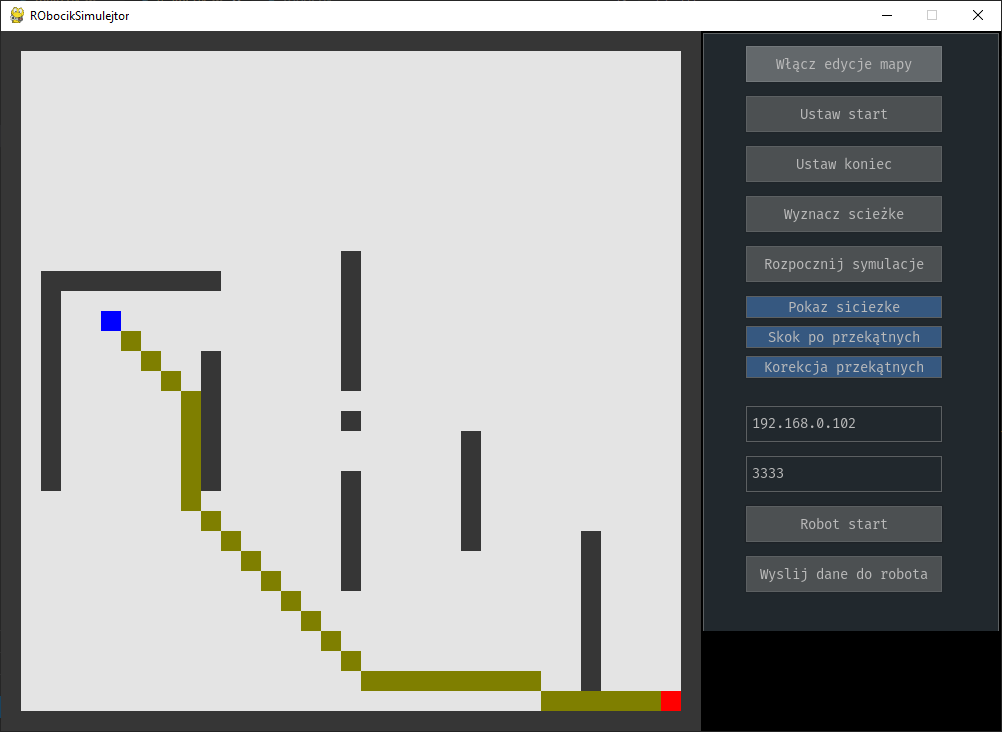
\includegraphics[width=9cm]{pages/testy/zdjecia/test3_ekualides_k10.png}
	\caption{Wyznaczona ścieżka, funkcja Eukalidesowa k=10}
\end{figure}
\textbf{Wzmocnienie k=1.41}

\begin{figure}[H]
	\centering
	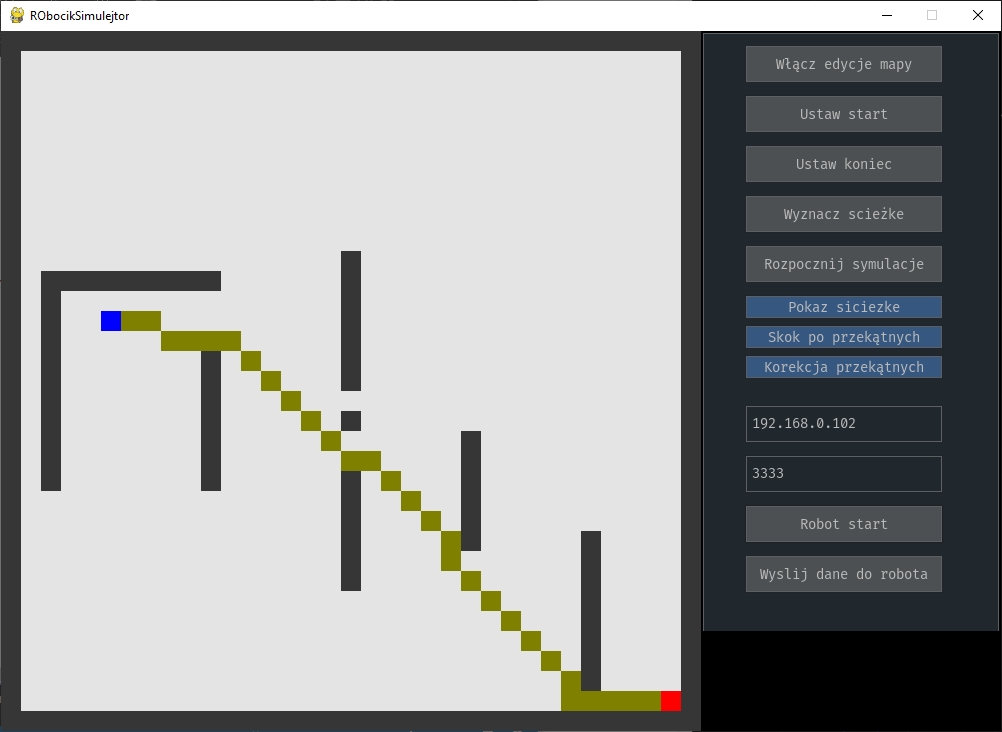
\includegraphics[width=9cm]{pages/testy/zdjecia/test3_ekualides_k141.png}
	\caption{Wyznaczona ścieżka, funkcja Eukalidesowa k=1.41}
\end{figure}

\subsubsection{Metryka miejska}
Kolejny test przeprowadzi wpływ metryki miejskiej opisanej wzorem nr. \eqref{Eq:heuresticManhattanu}

\begin{figure}[H]
	\centering
	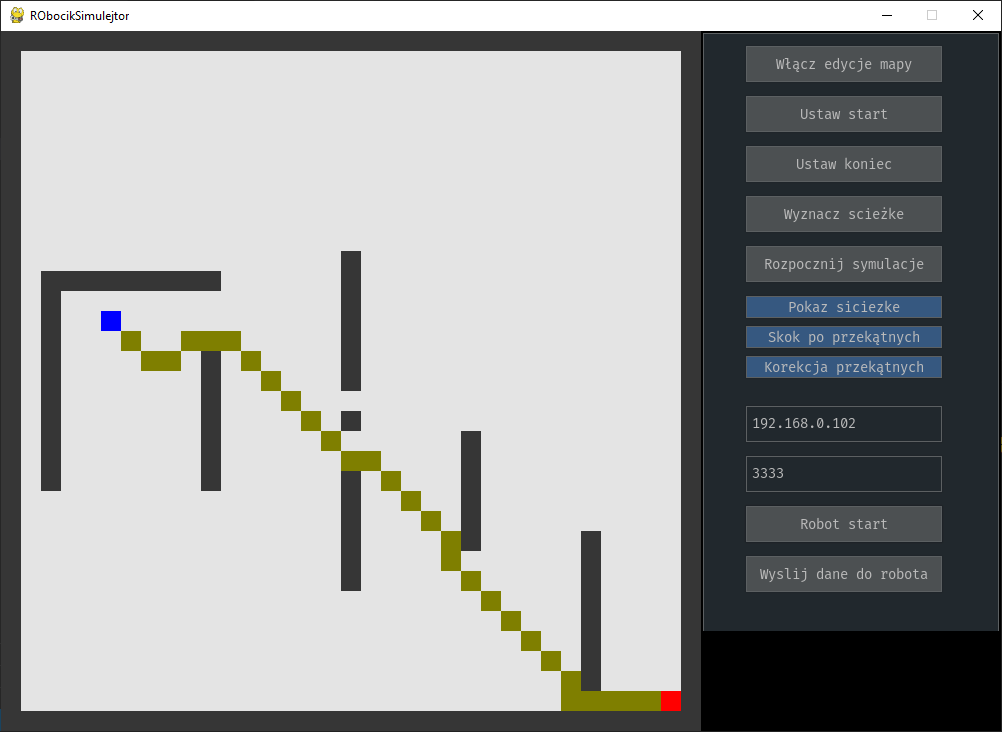
\includegraphics[width=9.5cm]{pages/testy/zdjecia/test3_taxi.png}
	\caption{Wyznaczona ścieżka, metryka miejska}
\end{figure}

\subsubsection{Dystans oktalny}
Ostatnie sprawdzona heurestyka implementuje dystans oktalny opisany wzorem nr. \eqref{Eq:heuresticOctileDistance}
\begin{figure}[H]
	\centering
	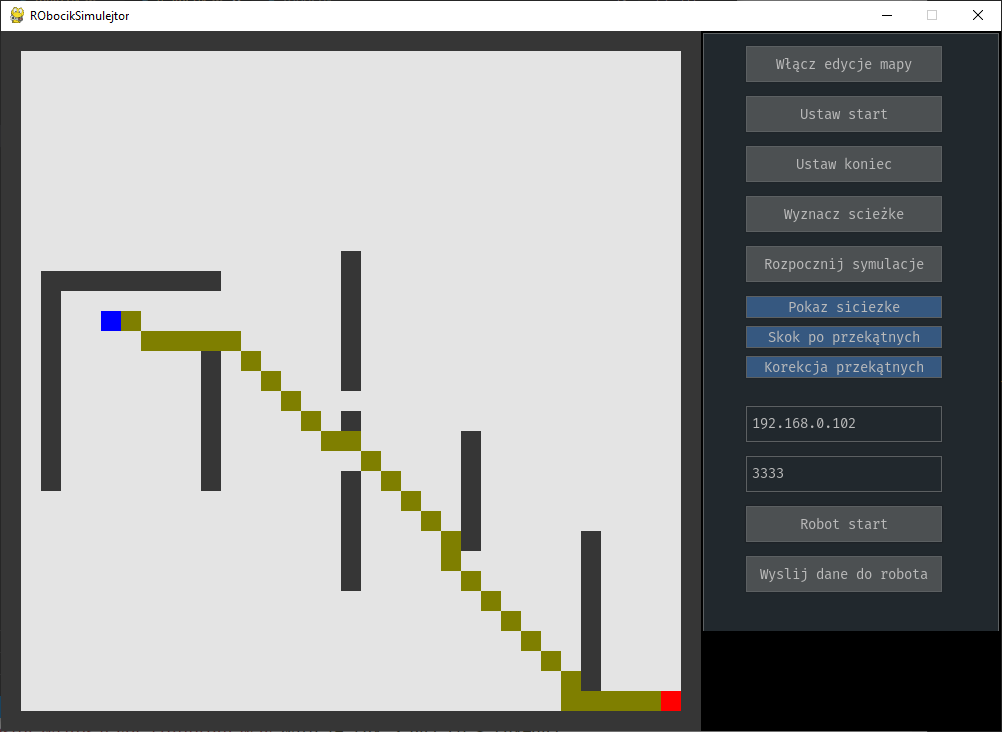
\includegraphics[width=9.5cm]{pages/testy/zdjecia/test3_H_przek.png}
	\caption{Wyznaczona ścieżka, dystans oktalny}
\end{figure}

Jak widać na powyższych zrzutach ekranu funkcje heurestyczne mają bardzo duży wpływ na wygenerowaną trasę i jej wybór może być 
uzależniony od środowiska, w którym porusza się robot. W tym przypadku funkcja Eukalidesowa ze wzmocnieniem 1.41 jest optymalna, 
generuję najkrótszą ścieżkę z długimi prostymi odcinkami co w przypadku realnego robota przyśpieszy przejazd.

\subsection{Test komunikacji z fizycznym robotem}
Poniższy test ma na celu sprawdzenie komunikacji pomiędzy zbudowanym robotem a programem do sterowania. 
Aby przeprowadzić test, został napisany prosty graficzny program pozwalający na ręczne sterowanie robotem. 
Po za nim istnieje konsola z możliwością wprowadzania i wysyłania komend.
W pierwszej kolejności należy poznać adres sieciowy jaki robot dostał od serwera DHCP. Aby to zrobić 
należy podłączyć mikrkontroler do komputera poprzez kabel usb i zainstalowaną przejściówkę USB-UART. 
Po uruchomieniu monitora odczytującego dane ze wskazanego portu, można odczytać adres. 
\begin{figure}[H]
	\centering
	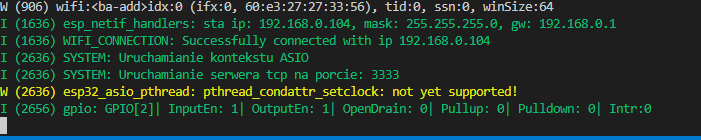
\includegraphics[width=13cm]{pages/testy/zdjecia/testSiec/idfMonitorIP.png}
	\caption{Odczytany adres IP}
\end{figure}
W następnym kroku możemy połączyć się przy pomocy konsoli lub dedykowanego programu. 
\begin{figure}[H]
	\centering
	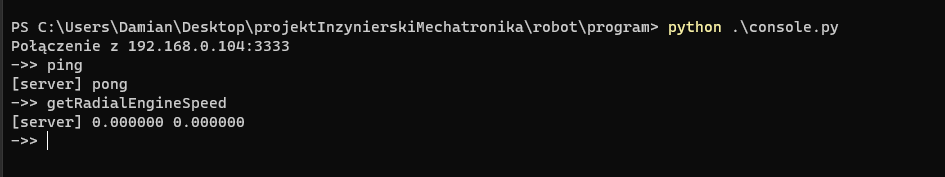
\includegraphics[width=10cm]{pages/testy/zdjecia/testSiec/testSiecKonsolePing.png}
	\caption{Testowe połączenie z konsoli}
\end{figure}

\begin{figure}[H]
	\centering
	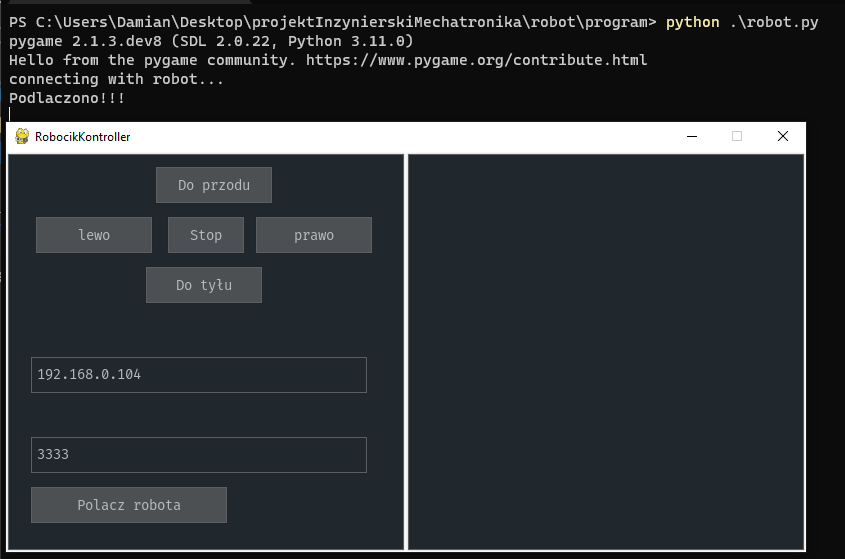
\includegraphics[width=10cm]{pages/testy/zdjecia/testSiec/testSterowanieReczne.png}
	\caption{Testowe połączenie do sterowania ręcznego}
\end{figure}

Po połączeniu z robotem możliwe jest ręczne sterowanie przy pomocy dedykowanych przycisków lub klawisze w,s,a i d.
Jeżeli wprowadzony adres ip jest błędny, w konsoli pojawi się odpowiedni komunikat opisujący błąd. 